\section{HTTP Method Request}
\subsection{Pengertian HTTP Method Request}
Protokol HTTP adalah protokol permintaan atau respon. Klien mengirimkan permintaan keserver dalam bentuk metode permintaan, URL, dan versi protokol, diikuti oleh pesan seperti MIME yang berisi perubahan permintaa, informasi klien, dan kemungkinan onten tubuh melalui koneksi dengan server\cite{wyler2005aggressive}. Protokol ini sangat ringan serta generik dan tidak berstatus sehingga dapat dipergunakan oleh tipe dokumen apa saja. Method adalah sekumpulan kode yang diberi namma, untuk merujuk kesekumpulan kode yang ada kemuadian digunakan sebuah nama yang disebut dengan nama method. Method sendiri mempunyai parameter sebagai input (masukan) dan nilai kembalian sebagai output (keluaran). Request adalah permiintaan dimana fungsi ini digunakan sebagai istilah ataupun kinerja dalam pengembalian nilai dari masukan yang dieksekusi.

Berdasarkan beberapa penjelasann diatas, maka untuk pengertian dari HTTP Method Request sendiri merupakan seperangkat metode permintan untuk menunjukkan tindakan yang diinginkan yang akan dilakukan untuk sumber daya tertentu. Meskipun mereka juga bisa menjadi kata benda, metode permintaan ini kadang-kadang disebut sebagai verba HTTP. Masing-masing menerapkan semantik yang berbeda, namun beberapa fitur umum digunakan bersama oleh mereka adalah misalnya Metode pertmintaan dapat berupa safe, idempotent, atau cacheable.

\subsection{Jenis-jenis HTTP Method Request}
\begin{enumerate}
  \item GET : akan dijelaskan pada point berikutnya.
  \item HEAD : Metode HEAD meminta tanggapan yang identik dengan permintaan GET, namun tanpa respon body.
  \item POST : Metode POST digunakan untuk mengirimkan entitas ke sumber daya yang ditentukan, sering menyebabkan perubahan pada keadaan atau efek samping pada server.
  \item PUT : Metode PUT menggantikan semua representasi terkini dari sumber target dengan muatan permintaan.
  \item DELETE : Metode DELETE akan menghapus sumber daya yang ditentukan
  \item CONNECT : Metode CONNECT menetapkan terowongan keserver yang diidentifikasi oleh sumber target.
  \item OPTIONS : Metode OPTIONS digunakan untuk menggambarkan opsi komunikasi untuk sumber target.
  \item TRACE : metode TRACE ini yaitu untuk melakukan tes pesan loop-back disepanjang jalan menuju sumber daya target.
  \item PATCH : Metode PATCH digunakan untuk menerapkan modifikasi sebagian pada sumber daya.
\end{enumerate}

\subsection{Penjelasan Lengkap HTTP Get Method}
Metode GET digunakan untuk meminta representasi suber daya yang ditentukan. permintaan menggunakan Get seharusnya hanya mengambil data. GET adalah salah satu metode HTTP yang paling umum digunakan baik dalam pengimplementasian biasa ataupun sudah dalam bentuk pengujian. Hal yang harus diperhatikan dalam Method Get yaitu :
\begin{itemize}
  \item Permintaan GET dapat di-cache.
  \item Permintaan GET tetap ada dalam riwayat browser.
  \item Permintaan GET dapat ditandai.
  \item Permintaan GET tidak boleh digunakan saat berurusan dengan data sensitif.
  \item Permintaan GET memiliki batasan panjang.
  \item Permintaan GET hanya digunakan untuk meminta data (tidak dimodifikasi).
  \item Permintaan GET dibatasi oleh panjang string sebanyak 2047 karakter.
  \item Permintaan GET memungkinkan pengunjung langsung memasukkan nilai variable pada form proses.
  \item Variabel diambil dengan \$\_REQUEST[“nama”] atau \$\_GET[“nama”]
\end{itemize}

\subsection{Pembacaan HTTP Get Method}
Data dikirimkan dalam HTTP Request dalam dua cara, tergantung dari method yang dikirimkan, yaitu :
\begin{enumerate}
  \item Melalui URL, dengan parameter yang diberikan. Digunakan oleh GET.
  \item Melalui entity body dalam HTTP Request. Digunakan untuk POST dan PUT.
\end{enumerate}

Pada prakteknya terdapat satu cara lagi untuk mengirimkan data, yaitu melalui cookie, tetapi penggunaan cookie tidak akan terlalu efektif karena cookie dirancang untuk menyimpan data status pengguna.

\subsection{Pembacaan Data pada URL}
Pembacaan data yang dikirimkan melalui URL biasanya dilakukan untuk request dengan method GET. Untuk melihat bagaimana GET mengirimkan data, kita terlebih dahulu harus mengerti tentang sintaks penulisan URL. Secara umum, sebuah URL memiliki sintaks seperti berikut :
\lstinputlisting[caption=Contoh kode untuk schema,label={lst:schema}]{src/10/schema.py}
Apa makna dari setiap bagian dari URL yang dijelaskan pada \ref{lst:schema}? Pada tabel \ref{table:schema}, anda dapat melihat makna dan maksud dari contoh URL yang telah diberikan.
\begin{table}[]
\caption{Penjelasan Schema}
\centering
\begin{tabular}{|l|l|l|}
\hline
Nama & Deskripsi & Harus ada ?\\ \hline
schema & Protokol yang digunakan & Ya\\ \hline
user & Nama pengguna & Tidak\\ \hline
password & Password untuk nama pengguna & Tidak\\ \hline
hots & Hostname atau IP & Ya\\ \hline
port & \begin{tabular}[c]{@{}l@{}}Port yang akan diakses. Beberapa atau sebagian\\ protokol memiliki port standar yaitu seperti HTTP = 80\end{tabular} & Tergantung Protokol\\ \hline
paht & Lokasi data pada server & Tergantung Protokol\\ \hline
query & \begin{tabular}[c]{@{}l@{}}Digunakan untuk mengirimkan \\ parameter kepada aplikasi.\end{tabular} & Tidak\\ \hline
fragment & \begin{tabular}[c]{@{}l@{}}Nama dari bagian tertentu pada \\ data (misalnya : judul pada buku)\end{tabular} & Tidak\\ \hline
\end{tabular}
\label{table:schema}
\end{table}

\section {Mekanisme HTTP Method Request}
\subsection{Mekanisme / Alur kerja HTTP Get Method}
Mekanisme adalah suatu rangkaian kerja sebuah alat yang digunakan dalam menyelesaikan sebuah masalah yang berkaitan dengan proses kerja, tujuannya untuk menghasilkan hasil yang mekasimal serta mengurangi datangnya atau munculnya kegagalan. untuk mekanisme HTTP Get Method sendiri dapat diperhatikan sebagai berikut :
\begin{enumerate}
  \item Silahkan membuat dan membangun sebuah URL API.
  \item Didalam URL API (endpoint) tersebut kita akan menggunakan fungsi Method Get.
  \item Kemudian didalam endpoint tersebut akan difungsikan inputan.
  \item Inputan tersebut kemudian akan meghasilkan output (keluaran) dari Metgod GET tersebut.
  \item Secara sederhana, garis besar mekanisme atau alur kerja Method Get nampak seperti penjelasan diatas.
  \item Untuk tutorial pembangunan endpoint seperrti pada point kedua akan dijelaskan pada point selanjutnya.
\end{enumerate}

\section {Contoh URL HTTP Get Method}
Untuk pemberian contoh ini akan dibarengin dengan tutorial pembangunannya, jadi diharapkan teman-teman dapat dengan mudah memahami dan mudah dalam mengikuti contoh yang diberikan. Berikut tutorialnya :
\begin{enumerate}
  \item Endpoint adalah perangkat komputasi jarak jauh yang berkomunikasi bolak-balik dengan jaringan yang terhubung dengannya. Fungsi-fungsi yang dipergunakan yaitu sebagai contoh berikut :
      \begin{itemize}
        \item Fungsi 1 : LoadData.py yaitu membaca file CSV.
            \lstinputlisting[caption=Contoh kode untuk membaca file CSV,label={lst:LoadData}]{src/10/LoadData.py}
        \item Fungsi 2 : Getalldata.py yaitu untuk menampilkan semua data dari file CSV.
            \lstinputlisting[caption=Contoh kode untuk menampilkan semua data dari file CSV,label={lst:GetAllData}]{src/10/GetAllData.py}
        \item Fungsi 3 : Getcolumn.py yaitu untuk menampilkan data dari kolom tertentu.
            \lstinputlisting[caption=Contoh kode untuk menampilkan data dari kolom,label={lst:Getcolumn}]{src/10/Getcolumn.py}
        \item Fungsi 4 : Gettopfive.py yaitu untuk menampilkan 5 data teratas dan terbawah.
            \lstinputlisting[caption=Contoh kode untuk menampilkan 5 data teratas dan terbawah,label={lst:Gettopfive}]{src/10/Gettopfive.py}
        \item Fungsi 5 : Sorting.py yaitu untuk mengurutkan data dari yang terbesar ke yang terkecil dan sebaliknya.
            \lstinputlisting[caption=Contoh kode untuk mengurutkan data,label={lst:Sorting}]{src/10/Sorting.py}
        \item Fungsi 6 : Convertjson.py yaitu untuk mengganti data kedalam format Json.
            \lstinputlisting[caption=Contoh kode untuk mengganti data,label={lst:Convertjson}]{src/10/Convertjson.py}
        \item Fungsi 7 : Deletecolumn.py yaitu untuk menghapus kolom tertentu.
            \lstinputlisting[caption=Contoh kode untuk menghampus kolom tertentu,label={lst:Deletecolumn}]{src/10/Deletecolumn.py}
        \item Fungsi 8 : Deletealldata.py yaitu untuk Menghapus semua data pada file CSV.
            \lstinputlisting[caption=Contoh kode untuk menghapus semua data,label={lst:Deletealldata}]{src/10/Deletealldata.py}
        \item Fungsi 9 : Insertdata.py yaitu untuk menambahkan data.
            \lstinputlisting[caption=Contoh kode untuk menambah data,label={lst:Insertdata}]{src/10/Insertdata.py}
        \item Fungsi 10 : Getinfo.py yaitu untuk Menampilkan data csv namun dengan format json bawaan dari library pandas yang akan berupa deskripsi.
            \lstinputlisting[caption=Contoh kode untuk Menampilkan data csv,label={lst:Getinfo}]{src/10/Getinfo.py}
        \item Fungsi 11 : Getrow.py yaitu untuk Menampilkan seluruh jumlah baris.
            \lstinputlisting[caption=Contoh kode untuk Menampilkan seluruh jumlah baris,label={lst:Getrow}]{src/10/Getrow.py}
        \item Fungsi 12 : Getrowfield.py yaitu untuk Menampilkan data perbaris sesuai dengan kolom yang diiginkan.
            \lstinputlisting[caption=Contoh kode untuk Menampilkan data perbaris,label={lst:Getrowfield}]{src/10/Getrowfield.py}
        \item Fungsi 13 : Updatedata.py yaitu untuk Mengubah data berdasarkan index id.
            \lstinputlisting[caption=Contoh kode untuk Mengubah data berdasarkan index id,label={lst:Updatedata}]{src/10/Updatedata.py}
        \item Fungsi 14 : Deletedata.py yaitu untuk Menghapus data berdasarkan index id.
            \lstinputlisting[caption=Contoh kode untuk Menghapus data berdasarkan index id,label={lst:Deletedata}]{src/10/Deletedata.py}
        \item Fungsi 15 : Getrowjson.py yaitu untuk Mengubah data menjadi Json.
            \lstinputlisting[caption=Contoh kode untuk Mengubah data menjadi Json,label={lst:Getrowjson}]{src/10/Getrowjson.py}
        \item Fungsi 16 : Getalldatajson.py yaitu untuk Menampilkan seluruh data dalam bentuk format Json.
            \lstinputlisting[caption=Contoh kode untuk Menampilkan seluruh data,label={lst:Getalldatajson}]{src/10/Getalldatajson.py}
        \item Fungsi 17 : Amountdata.py yaitu untuk Menghitung jumlah data secara keseluruhan dari kolom dan baris.
            \lstinputlisting[caption=Contoh kode untuk Menghitung jumlah data,label={lst:Amountdata}]{src/10/Amountdata.py}
        \item Fungsi 18 : Getcolumncount.py yaitu untuk Menghitung jumlah kolom pada file.
            \lstinputlisting[caption=Contoh kode untuk Menghitung jumlah kolom,label={lst:Getcolumncount}]{src/10/Getcolumncount.py}
        \item Fungsi 19 : Getrowcount.py yaitu untuk Menghitung jumlah baris pada file.
            \lstinputlisting[caption=Contoh kode untuk Menghitung jumlah baris,label={lst:Getrowcount}]{src/10/Getrowcount.py}
        \item Fungsi 20 : Reloaddata.py yaitu untuk Mengembalikan nilai data.
            \lstinputlisting[caption=Contoh kode untuk Mengembalikan nilai data,label={lst:Reloaddata}]{src/10/Reloaddata.py}
      \end{itemize}

 \subsection{Endpoint 1 (URL API / Dataset)}
  Pembatasan pertama ialah dari Endpoint 1 dimana URL API nya yaitu dataset. Silahkan tuliskan code dibawah sebagai contoh pertama :
  \lstinputlisting[caption=Contoh kode untuk URL API,label={lst:MethodGetfromEndpoint}]{src/10/MethodGetfromEndpoint.py}

  Pada tabel code diatas dapat dilihat bahwa fungsi yang digunakn ialah dataset dimana data set dilakukan pemaggilan fungsi yang ada di file-file yang telah di import. Seperti yang bisa dilihat bahwa pada fungsi dataset direalisasikan dengan metode GET, POST dan DELETE jadi disesuaikan dengan fungsi pada file-file yang dihubungkan atau dipanggil kedalam fungsi dataset. Yang akan dibahas disini adalah MEthod GETnya saja. Tutorialnya sebagai berikut :
  \begin{itemize}
    \item Setelah melakukan perintah \ref{lst:MethodGetfromEndpoint}
    \item Kemudian masukkan perintah yang sesuai
    \item Pendefinisian endpoint dataset
    \item Definisikan request atau permintaan metode yang digunakan. Ada Get 
    \item Pada Method GET : Silahkan masukkan beberapa argument yang akan diolah.
    \item Argumentnya ialah parameter field, topfive, sort dan format
    \item Penjelasan Parameter :
        \subitem All : Mengambil semua data dari file csv
        \subitem Field : Mengambil data berdasarkan parameter field yaitu ada RawValue, sign dan daya
        \subitem Topfive : Mengambil 5 data berdasarkan data paling atas dan 5 data paling bawah
        \subitem Sort : Mengambil data dan diurutkan sesuai dengan urutan ascending (kecil ke besar) dan descending (besar ke kecil)
        \subitem Format : Menampilkan data dengan format tulisan JSON dan Raw
    \item Selanjutnya pastikan setiap argument memberikan respon sesuai dengan fungsi masing-masing 
    \item Kemudian reloaddata akan menampilkan data terbaru setelah dilakukan perintah delete
    \item Silahkan uji endpointnya sesuai dengan parameter tersebut menggunakan POSTMAN maka hasilnya akan seperti berikut :
        
  \end{itemize}
\end{enumerate}

\begin{itemize}
\item HASIL PENGUJIAN ( Fungsi Dataset, method: GET ):
\end{itemize}

\begin{enumerate}
\item Menampilkan data secara keseluruhan ( /dataset ) seperti pada gambar \ref{fig:hujifd1}.
\begin{figure}[!htbp]
	\centerline{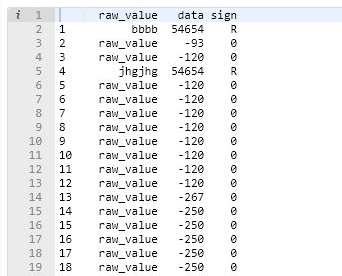
\includegraphics[width=0.85\textwidth]{figures/10/hujifd1.PNG}}
	\caption{Hasil Pengujian 1 fungsi dataset (GET)}
	\label{fig:hujifd1}
\end{figure}

\item Menampilkan data sesuai dengan field yang dimasukkan (/dataset?field=data) seperti pada gambar \ref{fig:hujifd2}.
\begin{figure}[!htbp]
	\centerline{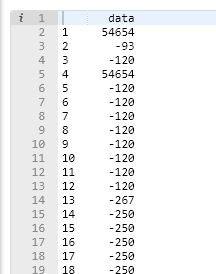
\includegraphics[width=0.85\textwidth]{figures/10/hujifd2.PNG}}
	\caption{Hasil Pengujian 2 fungsi dataset (GET)}
	\label{fig:hujifd2}
\end{figure}

\item Menampilkan data sesuai dengan field yang dimasukkan (/dataset?field=raw\_value) seperti pada gambar \ref{fig:hujifd3}.
\begin{figure}[!htbp]
	\centerline{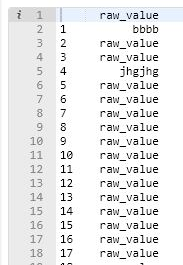
\includegraphics[width=0.85\textwidth]{figures/10/hujifd3.PNG}}
	\caption{Hasil Pengujian 3 fungsi dataset (GET)}
	\label{fig:hujifd3}
\end{figure}

\item Menampilkan data dalam bentuk Json ( /dataset?format=json) seperti pada gambar \ref{fig:hujifd4}.
\begin{figure}[!htbp]
	\centerline{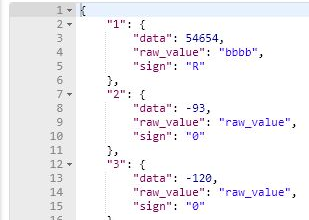
\includegraphics[width=0.85\textwidth]{figures/10/hujifd4.PNG}}
	\caption{Hasil Pengujian 4 fungsi dataset (GET)}
	\label{fig:hujifd4}
\end{figure}

\item Menampilkan 5 data teratas ( /dataset?topfive=first ) seperti pada gambar \ref{fig:hujifd5}.
\begin{figure}[!htbp]
	\centerline{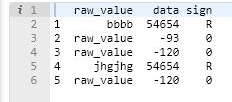
\includegraphics[width=0.85\textwidth]{figures/10/hujifd5.PNG}}
	\caption{Hasil Pengujian 5 fungsi dataset (GET)}
	\label{fig:hujifd5}
\end{figure}

\item Menampilkan data dengan urutan besar ke kecil (/dataset?field=data\&sort=descending)
seperti pada gambar \ref{fig:hujifd6}.
\begin{figure}[!htbp]
	\centerline{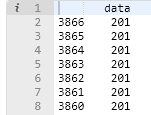
\includegraphics[width=0.85\textwidth]{figures/10/hujifd6.PNG}}
	\caption{Hasil Pengujian 6 fungsi dataset (GET)}
	\label{fig:hujifd6}
\end{figure}

\item Menampilkan 5 data teratas ( /dataset?topfive=first ) seperti pada gambar \ref{fig:hujifd7}.
\begin{figure}[!htbp]
	\centerline{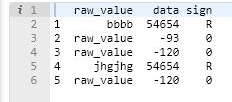
\includegraphics[width=0.85\textwidth]{figures/10/hujifd7.PNG}}
	\caption{Hasil Pengujian 7 fungsi dataset (GET)}
	\label{fig:hujifd7}
\end{figure}

\item Menampilkan data dengan urutan besar ke kecil (/dataset?field=data\&sort=descending) seperti pada gambar \ref{fig:hujifd8}.
\begin{figure}[!htbp]
	\centerline{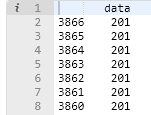
\includegraphics[width=0.85\textwidth]{figures/10/hujifd8.PNG}}
	\caption{Hasil Pengujian 8 fungsi dataset (GET)}
	\label{fig:hujifd8}
\end{figure}
\end{enumerate}

\subsection{Endpoint 2 ( URL API : /dataset/jumlah )}
Pembahasan selanjutnya yaitu tutorial untuk pembuatan endpoint kedua ( /dataset/jumlah ). Silahkan tuliskan code seperti pada listing \ref{lst:mge}:
\lstinputlisting[caption=Method Get dari Endpoint : URL API /dataset/jumlah,label={lst:mge}]{src/10/mge.py}
Pada listing \ref{lst:mge} ada fungsi jumlah, pada fungsi ini di panggil lah fungsi jumlah\_data yang bisa dieksekusi dengan beberapa nilai seperti misalnya kolom, row dan lain-lain. Bisa dilihat di bagian alur manipulasi data. 
Tutorial :
\begin{enumerate}
\item Silahkan melanjutkan contoh file diatas
\item Masukkan endpoint dataset/jumlah
\item Terapkan method Get : dengan fungsi jumlah dimana di dalamnya terdapat argument untuk parameter from ( row dan column )
\item Penjelasan Parameter From :
\begin{itemize}
\item Column		:Akan mengambil dan menampilkan jumlah kolom sesuai dengan kolom yang ada pada file CSV yang dieksekusi.
\item Row		:Akan mengambil dan menampilkan jumlah baris sesuai dengan baris yang ada pada file CSV yang dieksekusi.
\end{itemize}
\item Kemudian pada argument/parameter from tersebut, fungsi jumlah\_data dijadikan sebagai respon
\item Fungsi jumlah\_data akan menghitung berapa banyak jumlah baris dan kolom pada data ( tertentu, sesuai dengan parameternya yang di get)
\item Kemudian apabila pengeksekusian tanpa dibarengi dengan argument/parameter maka akan menampilkan jumlah keseluruhan.
\end{enumerate}

\begin{itemize}
\item HASIL PENGUJIAN ( Fungsi Dataset/jumlah , method: GET ):
\end{itemize}
\begin{enumerate}
\item Menampilkan jumlah data secara keseluruhan ( /dataset/jumlah ) seperti pada gambar \ref{fig:hujifdj1}.
\begin{figure}[!htbp]
	\centerline{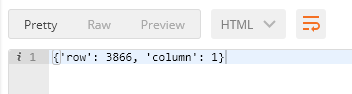
\includegraphics[width=0.85\textwidth]{figures/10/hujifdj1.PNG}}
	\caption{Hasil Pengujian 1 fungsi dataset/jumlah (GET)}
	\label{fig:hujifdj1}
\end{figure}

\item Menampilkan jumlah data row (/dataset/jumlah?from=row) seperti pada gambar \ref{fig:hujifdj2}.
\begin{figure}[!htbp]
	\centerline{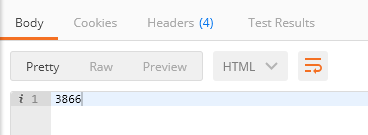
\includegraphics[width=0.85\textwidth]{figures/10/hujifdj2.PNG}}
	\caption{Hasil Pengujian 2 fungsi dataset/jumlah (GET)}
	\label{fig:hujifdj2}
\end{figure}

\item  Menampilkan jumlah data row (/dataset/jumlah?from=column) seperti pada gambar \ref{fig:hujifdj3}.
\begin{figure}[!htbp]
	\centerline{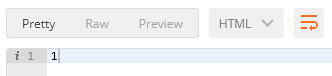
\includegraphics[width=0.85\textwidth]{figures/10/hujifdj3.PNG}}
	\caption{Hasil Pengujian 3 fungsi dataset/jumlah (GET)}
	\label{fig:hujifdj3}
\end{figure}
\end{enumerate}

\subsection{Endpoint 3 ( URL API : /dataset/<id> )}
Pembahasan selanjutnya yaitu tutorial untuk pembuatan endpoint ketiga ( /dataset/<id> ). Silahkan perhatikan dan ikuti file seperti pada listing \ref{lst:mege}:
\lstinputlisting[caption=Method Get dari Endpoint : URL API /dataset/<id>,label={lst:mege}]{src/10/mege.py}
Pada listing \ref{lst:mege} terdapat fungsi detail. Di dalam fungsi tersebut dipergunakan untuk pengeksekusian data memakai fungsi yang diperlukan penentuan index id. Jadi kebanyakan dari hasil fungsi yang dipanggil dan dihubungkan kedalam fungsi detail. 
Tutorial :
\begin{enumerate}
\item Silahkan melanjutkan contoh file diatas
\item Masukkan endpoint dataset/id
\item Terapkan method Get : dengan fungsi jumlah dimana di dalamnya terdapat argument untuk parameter field ( raw\_value, data, sign ) dan format ( json )
\item Penjelasan Parameter :
\begin{itemize}
\item All	:Menampilkan data sesuai index id yang dipanggil tanpa parameter tertentu.
\item Field	:Menampilkan dan mengambil data dari kolom tertentu dan disesuaikan dengan index id yang telah dipanggil
\item Format	:Menampilkan dan mengambil data dengan format tulisan JSON dan RAW sesuai dengan index id yang dipanggil.
\end{itemize}
\item Kemudian pada argument/parameter field tersebut, fungsi get\_row\_field dijadikan sebagai respon
\item Fungsi get\_row\_field akan mengambil data dari row tersebut sesuai dengan field yang dimasukkan 
\item Selanjutnya pada argument/parameter format, fungsi jsonify(get\_all\_data\_json) dijadikan sebagai respon
\item Fungsi get\_all\_data\_json akan mengambil data dari id tersebut dan ditampilkan dengan format json string. 
 \item Kemudian reload\_data akan menampilkan data terbaru setelah dilakukan perintah delete.
 \item Setelah semuanya selesai, maka tutorial untuk tahapan ini juga sudah berhasil.
\end{enumerate}
\begin{itemize}
\item HASIL PENGUJIAN ( Fungsi Dataset/<id>, method: GET ):
\end{itemize}
\begin{enumerate}
\item Menampilkan data berdasarkan id ( /dataset/<id>) seperti pada gambar \ref{fig:hujifdi1}.
\begin{figure}[!htbp]
	\centerline{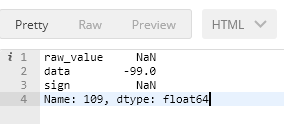
\includegraphics[width=0.85\textwidth]{figures/10/hujifdi1.PNG}}
	\caption{Hasil Pengujian 1 fungsi dataset/<id> (GET)}
	\label{fig:hujifdi1}
\end{figure}

\item Menampilkan data sesuai id dengan format json (/dataset/1?format=json) seperti pada gambar \ref{fig:hujifdi2}.
\begin{figure}[!htbp]
	\centerline{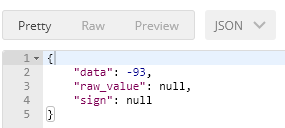
\includegraphics[width=0.85\textwidth]{figures/10/hujifdi2.PNG}}
	\caption{Hasil Pengujian 2 fungsi dataset/<id> (GET)}
	\label{fig:hujifdi2}
\end{figure}

\item Menampilkan data sesuai id dengan format raw (/dataset?format=raw) seperti pada gambar \ref{fig:hujifdi3}.
\begin{figure}[!htbp]
	\centerline{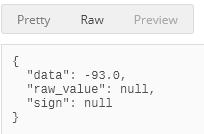
\includegraphics[width=0.85\textwidth]{figures/10/hujifdi3.PNG}}
	\caption{Hasil Pengujian 3 fungsi dataset/<id> (GET)}
	\label{fig:hujifdi3}
\end{figure}

Gambar 9.14. Hasil pengujian 3 fungsi dataset/<id> (GET)
\end{enumerate}

\subsection{Endpoint 4 ( URL API : /info )}
Pembahasan selanjutnya ialah untuk endpoint terakhir yaitu endpoint info. Silahkan perhatikan file dibawah kemudian silahkan anda ikuti seperti pada listing \ref{lst:mgei}:
\lstinputlisting[caption=Method Get dari Endpoint : URL API /dataset/info,label={lst:mgei}]{src/10/mgei.py}

Pada file ini cukup sederhana fungsinya yaitu hanya untuk mendapatkan data berupa deskripsi bawaan dari library ( bentuknya akan berbeda dari GET data sebelumnya )

Tutorial :
\begin{enumerate}
\item Silahkan melanjutkan contoh file diatas
\item Masukkan endpoint info
\item Terapkan method Get : dengan fungsi info diatas
\item Setelah itu silahkan eksekusi menggunakan CMD maka hasilnya akan sebagai berikut :
\end{enumerate}
\begin{itemize}
\item HASIL PENGUJIAN ( Fungsi info, method: GET ):
\end{itemize}
Menampilkan data berdasarkan info yang disimpan library pandas ( /info) seperti pada gambar \ref{fig:hujiinf}.
\begin{figure}[!htbp]
	\centerline{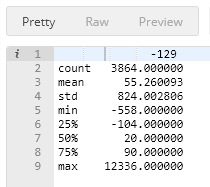
\includegraphics[width=0.85\textwidth]{figures/10/hujiinf.PNG}}
	\caption{Hasil Pengujian 1 fungsi dataset/info (GET)}
	\label{fig:hujiinf}
\end{figure}

\section {Mendapatkan Parameter GET Python Flask}
\subsection{Penjelasan Parameter GET Python Flask}
Parameter GET pada Python Flask ini saya lampirkan dan ujikan dalam bentuk file penuh dengan beberapa fungsi. File tersebut bernama Main.py. Untuk penerapan lebih dan contoh GETnya sudah saya tampilkan dan jelaskan sebelumnya pada point contoh URL GET. 
Namun, penggabungannya bersama Flask Python ada pada file ini. Silahkan diperhatikan penjelasan dan tutorialnya dan semoga dapat dimengerti. 

Namun sebelum melanjutkan tutorial silahkan pertama-tama kita harus memastikan beberapa hal yaitu :
\begin{enumerate}
\item Persiapan Python : Instalasi Python 3.6
Instalasi Python dapat ditemukan di penjelasan sebelumnya ( Sub Menu 1 ). Namun apabila masih belum paham dapat mengikuti langkah-langkah berikut:
\begin{itemize}
\item Pertama-tama silahkan download software dari python versi 3 di laptop anda.
\item Download python versi 3.6.3 dari situs web resminya yaitu https://www.python.org/
\item Silahkan sesuaikan dengan kapasitas laptop anda, bisa yang win 32 atau yang win 64 ( 32 bit / 64 bit )
\item Contoh downloadnya seperti pada gambar \ref{fig:inspy}.
\begin{figure}[!htbp]
	\centerline{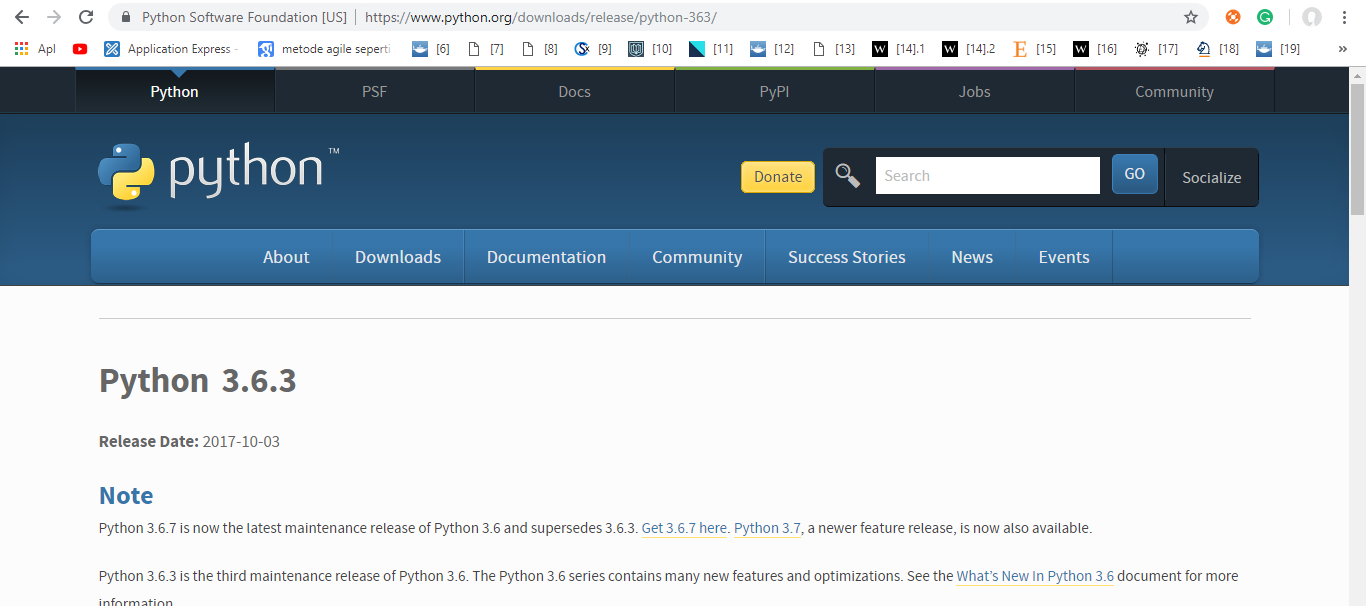
\includegraphics[width=0.85\textwidth]{figures/10/inspy.PNG}}
	\caption{Instalasi Python}
	\label{fig:inspy}
\end{figure}

\item Setelah berhasil melakukan pengunduhan/download aplikasi python tersebut, maka silahkan lakukan instalasi
\item Instalasi dapat dilakukan seperti instalasi biasa pada umumnya
\item Setelah selesai instalasi python, silahkan check di Command Prompt, apakah Pythonnya telah terbaca / running disesuaikan dengan laptop anda atau belum.
\item Contoh pengecekan di Command Prompt seperti pada gambar \ref{fig:pyc}.
\begin{figure}[!htbp]
	\centerline{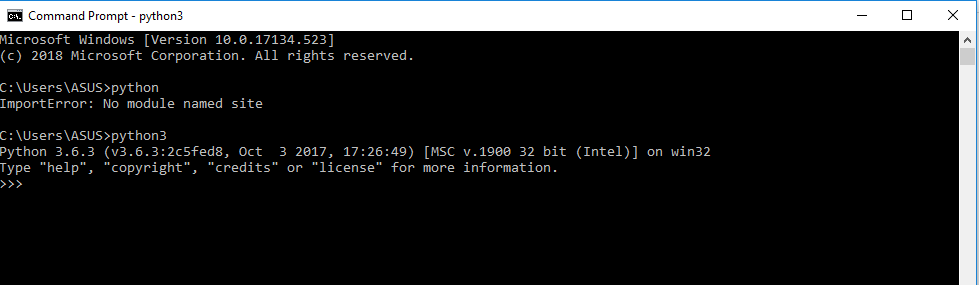
\includegraphics[width=0.85\textwidth]{figures/10/pyc.PNG}}
	\caption{Python CMD}
	\label{fig:pyc}
\end{figure}

\item Apabila tampilannya telah sesuai dengan contoh diatas, maka python anda siap digunakan. 
\item Pastikan python yang terbaca versi 3.6.3 atau bahkan belum ada sama sekali silahkan lakukan konfigurasi ini :
\begin{itemize}
\item Silahkan buka Control Panel anda
\item Pilih System and Security
\item Kemudian pilih lagi system
\item Lalu di bagian kiri tampilan ada sub menu Advanced system setting
\item Pada sub menu tersebut silahkan pilih button Environment Variabel
\item Silahkan ganti path dengan C:/Python36 dan C:/Python36/Scripts ( Lokasi anda menyimpan mentahan python yang telah anda install tadi )
\item Maka tampilannya akan seperti pada gambar \ref{fig:dme}.
\begin{figure}[!htbp]
	\centerline{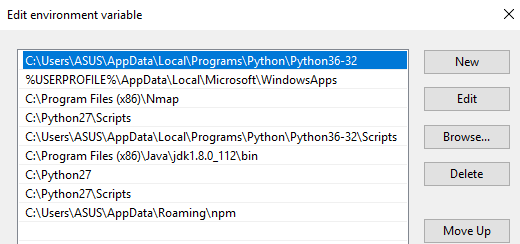
\includegraphics[width=0.85\textwidth]{figures/10/dme.PNG}}
	\caption{Device Manager ( Env )}
	\label{fig:dme}
\end{figure}

\item Jangan lupa untuk memasukkan script dari python sehingga benar-benar bisa terbaca untuk pipnya.
\item Silahkan klik button ok sampai selesai
\item Setelah itu, lakukan pengecekan ulang di Command Prompt maka hasilnya akan berubah menjadi versi 3.6.3 
\item Setelah semua tahap di atas selesai, maka silahkan lanjutkan ke tahap berikutnya
\end{itemize}
\end{itemize}

\item Persiapan Flask

Tutorial selanjutnya ialah kita akan menginstall Framework Flask di komputer/laptop kita sehingga bisa digunakan untuk tutorial selanjutnya. Untuk teman-teman ketahui flask sendiri merupakan microframework dari python, dengan penggunaannya, aktivas apapun yang kita lakukan baik pengolahan data dll akan terasa lebih mudah dan rapih, kurang lebih seperti itu.

Instalasi Flask dapat ditemukan di penjelasan sebelumnya ( Sub Menu 7 ). Namun apabila masih belum paham dapat mengikuti langkah-langkah berikut :
\begin{itemize}
\item Pertama-tama silahkan nyalakan laptop / komputer anda
\item Kemudian apabila komputer / laptop anda telah bisa digunakan silahkan buka web browser 
\item Web browser yang digunakan bisa Chrome. Mozilla Firefox dll sesuai dengan keinginan anda.
\item Selanjutnya pada web browser silahkan kunjungi website resmi berikut : https://pypi.org/project/Flask/
\item Pada website tersebut silahkan download Flask
\item Contohnya nampak seperti pada gambar \ref{fig:insfla}.
\begin{figure}[!htbp]
	\centerline{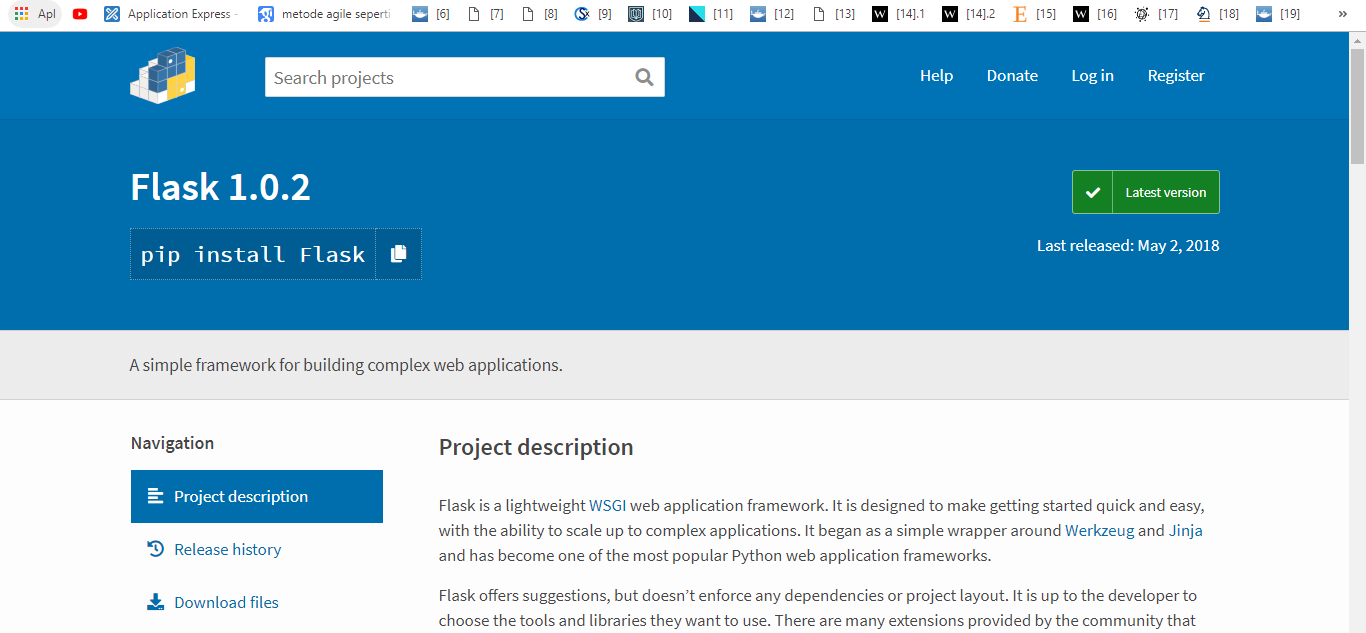
\includegraphics[width=0.85\textwidth]{figures/10/insfla.PNG}}
	\caption{Instalasi Flask}
	\label{fig:insfla}
\end{figure}

\item Setelah di download silahkan buka Command Prompt di komputer/laptop anda
\item Kemudian silahkan ketikkan perintah ( pip install flask )
\item Setelah mengetikkan perintah tersebut, silahkan tekan enter maka prosesnya akan belajar
\item Silahkan tunggu hasilnya
\item Hasilnya akan nampak seperti pada gambar \ref{fig:ifc}.
\begin{figure}[!htbp]
	\centerline{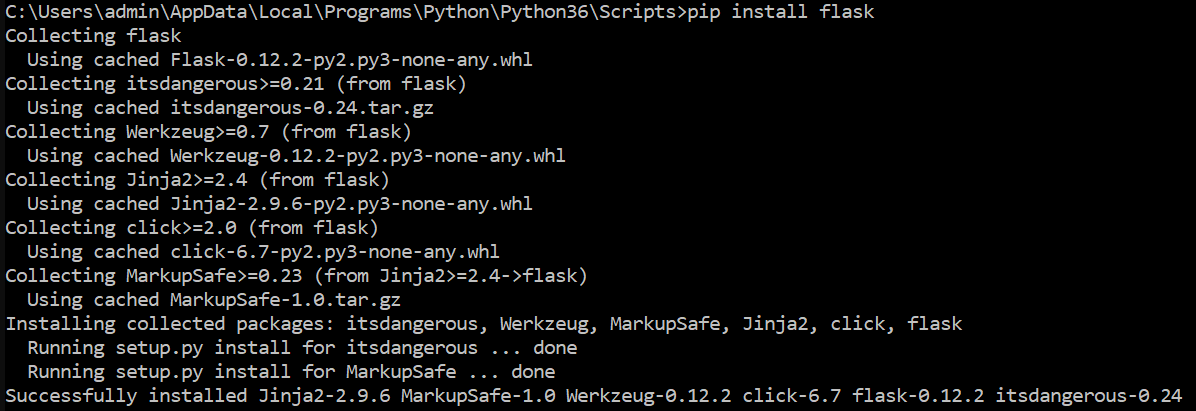
\includegraphics[width=0.85\textwidth]{figures/10/ifc.PNG}}
	\caption{Install Flask di CMD}
	\label{fig:ifc}
\end{figure}

\item Apabila tampilan pada proses di komputer/laptop anda telah nampak seperti gambar yang dicontohkan maka prosesnya berhasil
\item Dan apabila masih terjadi error maka silahkan lakukan kembali langkah-langkahnya, bisa saja anda melewatkan beberapa point pada tutorial ini
\item Setelah flasknya terpasang di komputer/laptop anda maka silahkan lanjutkan ke tutorial selanjutnya.
\end{itemize}

\item Persiapan Library Pandas ( untuk menyesuaikan dengan file CSV yang dieksekusi.

Tutorial selanjutnya ialah kita akan menginstall Library Pandas di komputer/laptop kita sehingga bisa digunakan untuk tutorial selanjutnya. Untuk teman-teman ketahui pandas sendiri merupakan library dari bahasa pemrograman Python. Library ini digunakan untuk pemrosesan data analitik. Mengapa kita gunakan? Karena memang pandas ini akan mengolah data analitik dari CSV file yang berisikan data sinyal gelombang otak yang kita baca dan tangkap dari aktifitas tertentu ( lampu sein saat bermotor ). Nah mari kita mulai:

Instalasi Pandas dapat ditemukan di penjelasan sebelumnya ( Sub Menu 7 ). Namun apabila masih belum paham dapat mengikuti langkah-langkah berikut :
\begin{itemize}
\item Pertama-tama silahkan nyalakan laptop / komputer anda
\item Kemudian apabila komputer / laptop anda telah bisa digunakan silahkan buka web browser 
\item Web browser yang digunakan bisa Chrome. Mozilla Firefox dll sesuai dengan keinginan anda.
\item Selanjutnya pada web browser silahkan kunjungi website resmi berikut : https://pypi.org/project/pandas/
\item Pada website tersebut silahkan download Pandas
\item Contohnya nampak seperti pada gambar \ref{fig:inspa}.
\begin{figure}[!htbp]
	\centerline{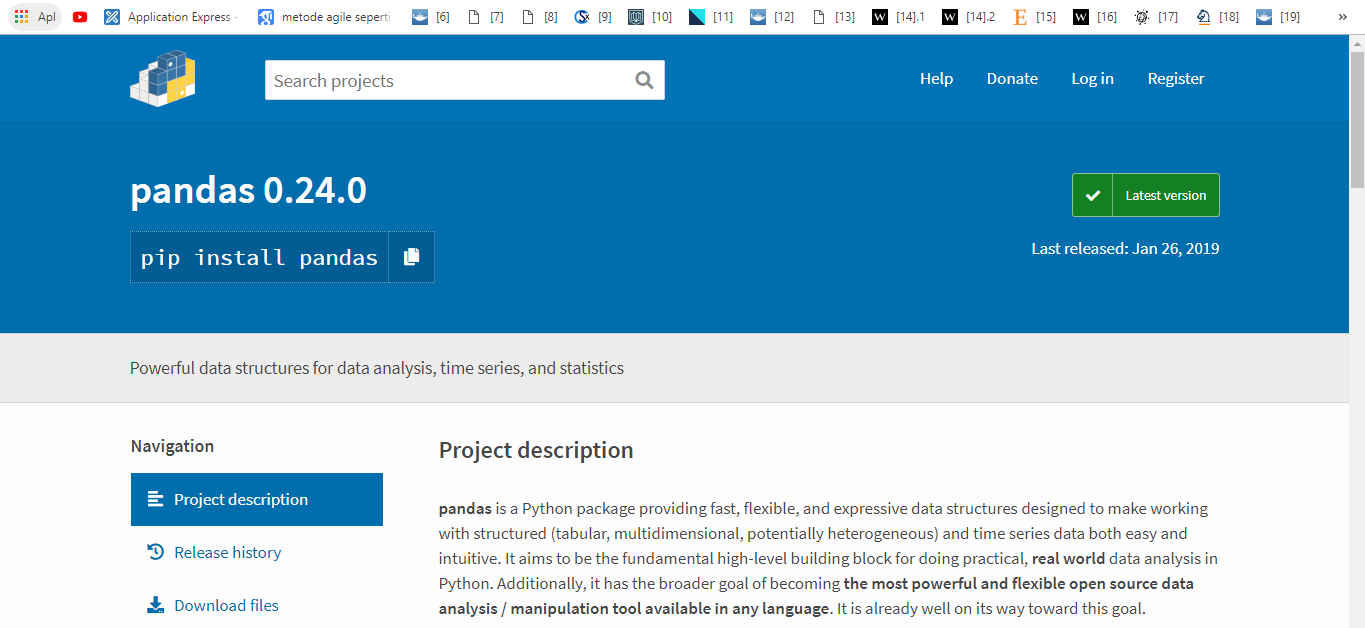
\includegraphics[width=0.85\textwidth]{figures/10/inspa.PNG}}
	\caption{Instalasi Pandas}
	\label{fig:inspa}
\end{figure}

\item Setelah di download silahkan buka Command Prompt di komputer/laptop anda
\item Kemudian silahkan ketikkan perintah ( pip install pandas )
\item Setelah mengetikkan perintah tersebut, silahkan tekan enter maka prosesnya akan belajar
\item Silahkan tunggu hasilnya
\item Hasilnya akan nampak seperti pada gambar \ref{fig:ipc}.
\begin{figure}[!htbp]
	\centerline{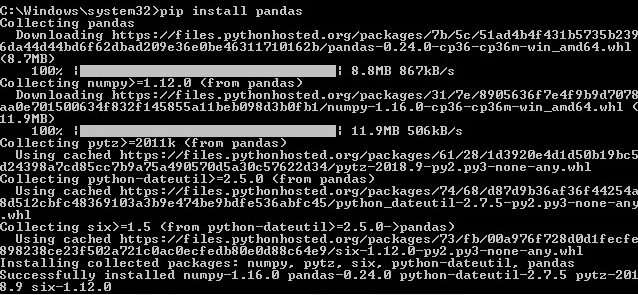
\includegraphics[width=0.85\textwidth]{figures/10/ipc.PNG}}
	\caption{Install Pandas di CMD}
	\label{fig:ipc}
\end{figure}

\item Apabila tampilan pada proses di komputer/laptop anda telah nampak seperti gambar yang dicontohkan maka prosesnya berhasil
\item Dan apabila masih terjadi error maka silahkan lakukan kembali langkah-langkahnya, mungkin anda melewatkan beberapa point pada tutorial ini
\item Setelah pandasnya terpasang di komputer/laptop anda maka silahkan lanjutkan ke tutorial selanjutnya
\end{itemize}
\end{enumerate}

Filenya yang akan dijadikan tutorial yaitu seperti pada listing \ref{lst:mpf}:
\lstinputlisting[caption=File Main.py Python Flask,label={lst:mpf}]{src/10/mpf.py}

Penjelasan Lengkap :
\begin{enumerate}
\item Penjelasan I : Main.py
\lstinputlisting[caption=Penjelasan I : Main.py,label={lst:pm1}]{src/10/pm1.py}

Listing \ref{lst:pm1} merupakan codingan untuk mendefinisikan framework flask, beberapa module yang digunakan untuk mengeksekusi fungsi seperti request, jsonify dan juga ada library pandas yang digunakan untuk pengeksekusian data analitik seperti file csv yang digunakan. Pada code juga dilakukan pemanggilan file-file yang di dalamnya telah terdapat masing-masing fungsi yang telah dijelaskan sebelumnya sehingga semuanya dapat dieksekusi dalam 1 framework Flask Python.
Langkah-langkah :
\begin{itemize}
\item Silahkan buka sublime anda
\item Kemudian buatlah file baru dengan nama Main.py
\item Kemudian silahkan masukkan perintah import
\item Perintah import apa saja? Silahkan mengimportkan perintah/file sesuai dengan contoh pada gambar
\end{itemize}

\item Penjelasan II : Main.py
\lstinputlisting[caption=Penjelasan II : Main.py,label={lst:pm2}]{src/10/pm2.py}

Listing \ref{lst:pm2}  dijelaskan bahwa file yang dieksekusi ialah Book1.csv kemudian variabel dataframenya akan memanggil fungsi load\_data yang di dalamnya juga didefinisikan variabel filename. Indexnya sendiri ialah 1. Untuk fungsi reload\_data memiliki variabel fname dan dfname .
\begin{itemize}
\item Silahkan lanjutkan pada file main.py
\item Kemudian masukkan perintah diatas
\item Variabel Filename disesuaikan dengan file yang akan diolah ( misal Book1.csv)
\item Kemudian jangan lupa masukkan variabel dataframe ( tentunya untuk pengolahan data secara keseluruhan )
\item Lalu, difungsikan juga reload\_data ( mengupdate data ketika ada perubahan )
\item Jangan lupa untuk menambahkan dataframe.to\_csv sehingga parameternya akan dipisahkan oleh perintah ( sep = “ : ” ) dengan index=false
\item Selanjutnya silahkan return variabel dataframe
\end{itemize}

\item Penjelasan III : Main.py
Penjelasan ini terdiri dari penjelasan untuk setiap endpoint dari Method GETnya.
\begin{itemize}
\item Endpoint 1 ( URL API : /dataset ): Telah dijelaskan pada point contoh URL Get. Halaman 7-14
\item Endpoint 2 ( URL API : /dataset/jumlah ): Telah dijelaskan pada point contoh URL Get. Halaman 7-14
\item Endpoint 3 ( URL API : /dataset/<id> ): Telah dijelaskan pada point contoh URL Get. Halaman 7-14
\item Endpoint 4 ( URL API : /info ): Telah dijelaskan pada point contoh URL Get. Halaman 7-14
\end{itemize}

\item Penjelasan IV : Main.py
\lstinputlisting[caption=Penjelasan IV : Main.py,label={lst:pm4}]{src/10/pm4.py}

Listing \ref{lst:pm4} difungsikan untuk mengeksekusi inputan yang telah dimasukkan kedalam flask yang menjadi body dari code tersebut yaitu Main.py . Kemudian ketika dijalankan hasilnya true maka aplikasinya akan jalan sesuai dengan yang seharusnya
\end{enumerate}

\section{Penanganan Error}
\subsection{Error 1}
\begin{enumerate}
\item Silahkan jalankan kembali CMD anda
\item Kemudian masuk ke Directory tempat anda menyimpan file main.py
\item Kemudian masukkan perintah berikut :
\verb|Env/scripts/activate|
\item Maksud dari Code tersebut ialah untuk mengaktifkan scriptnya python3
\item Maka hasilnya akan nampak seperti pada gambar \ref{fig:am2}.
\begin{figure}[!htbp]
	\centerline{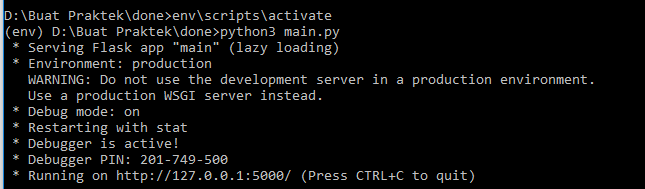
\includegraphics[width=0.85\textwidth]{figures/10/am2.PNG}}
	\caption{Aktivasi main.py 2 pada contoh kasus 3}
	\label{fig:am2}
\end{figure}

\item Apabila hasilnya seperti gambar diatas maka filenya telah berjalan dengan baik
\item Bisa dilihat, untuk URL APInya sudah muncul jadi silahkan copy dan buktikan menggunakan POSTMAN atau browser biasa.
\item Hasilnya seperti berikut, apabila dieksekusi sesuai endpoint.
\item Misalnya endpoint : dataset/<id>  seperti pada gambar \ref{fig:huji1}.
\begin{figure}[!htbp]
	\centerline{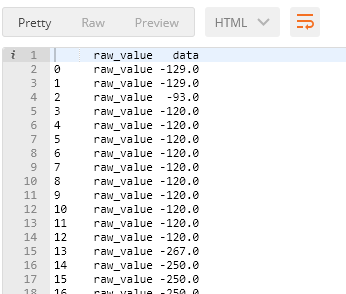
\includegraphics[width=0.85\textwidth]{figures/10/huji1.PNG}}
	\caption{Hasil pengujian 1 untuk error 9 pada contoh kasus 3}
	\label{fig:huji1}
\end{figure}

\item Kemudian apabila muncul ERROR seperti pada gambar \ref{fig:err1}.
\begin{figure}[!htbp]
	\centerline{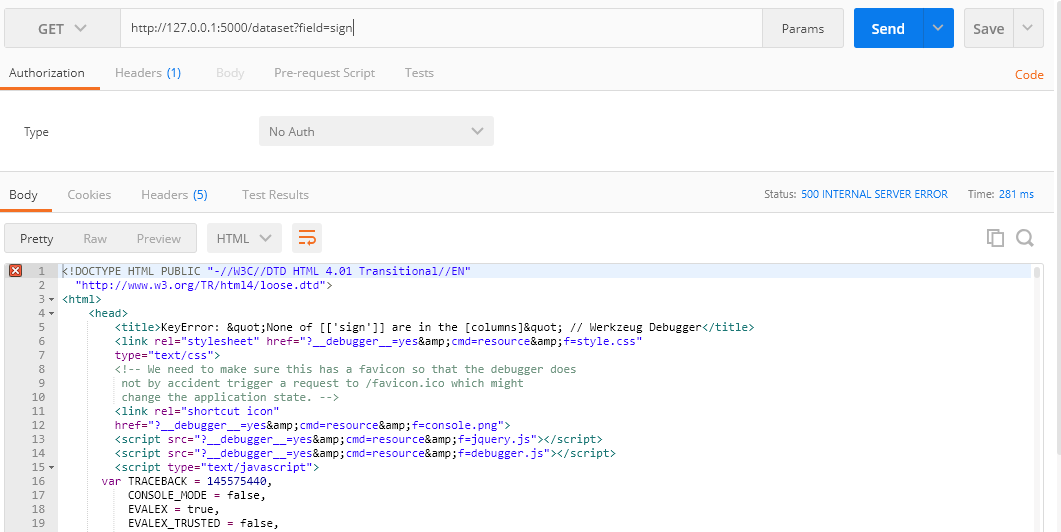
\includegraphics[width=0.85\textwidth]{figures/10/err1.PNG}}
	\caption{Error 1 untuk error 9 pada contoh kasus 3}
	\label{fig:err1}
\end{figure}

\item Maka tindakannya seperti berikut:
\begin{itemize}
\item Perhatikan terlebih dahulu request yang diminta
\item Request yang diminta yaitu field dengan parameter kolom sign
\item Silahkan diperiksa dulu apakah pada file yang ingin di get, kolom tersebut masih ada.
\item Apabila tidak ada, maka silahkan masukkan file baru yang ada kolom signnya
\item Kemudian silahkan jalankan kembali requestnya
\item Maka hasilnya akan nampak seperti pada gambar \ref{fig:huji2}.
\begin{figure}[!htbp]
	\centerline{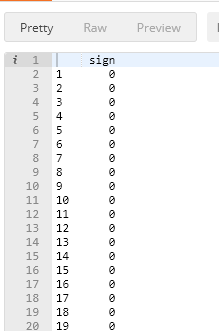
\includegraphics[width=0.85\textwidth]{figures/10/huji2.PNG}}
	\caption{Hasil pengujian 2 untuk error 9 pada contoh kasus 3}
	\label{fig:huji2}
\end{figure}
\end{itemize}
\end{enumerate}

\subsection{Error 2}
\begin{enumerate}
\item Silahkan jalankan kembali CMD anda
\item Kemudian masuk ke Directory tempat anda menyimpan file main.py
\item Kemudian masukkan perintah berikut : \verb|Env/scripts/activate|
\item Maksud dari Code tersebut ialah untuk mengaktifkan scriptnya python3
\item Maka hasilnya akan nampak seperti pada gambar \ref{fig:am3}.
\begin{figure}[!htbp]
	\centerline{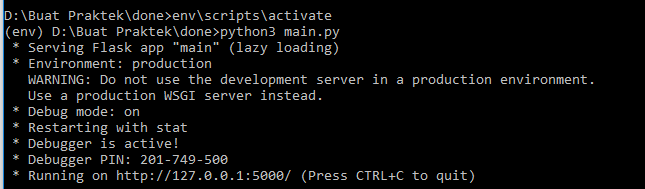
\includegraphics[width=0.85\textwidth]{figures/10/am3.PNG}}
	\caption{Aktivasi main.py 3 pada contoh kasus 3}
	\label{fig:am3}
\end{figure}

\item Apabila hasilnya seperti gambar diatas maka filenya telah berjalan dengan baik
\item Bisa dilihat, untuk URL APInya sudah muncul. Silahkan copy dan buktikan menggunakan POSTMAN atau browser biasa.
\item Hasilnya seperti berikut, apabila dieksekusi sesuai endpoint.
\item Misalnya endpoint : dataset seperti pada gambar \ref{fig:hu1}.
\begin{figure}[!htbp]
	\centerline{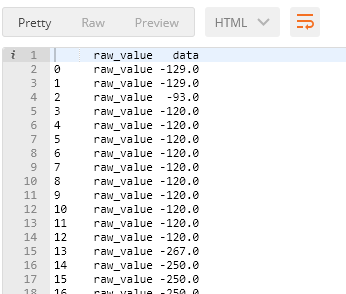
\includegraphics[width=0.85\textwidth]{figures/10/hu1.PNG}}
	\caption{Hasil pengujian 1 untuk error 10 pada contoh kasus 3}
	\label{fig:hu1}
\end{figure}

\item Kemudian apabila muncul ERROR seperti pada gambar \ref{fig:er1}.
\begin{figure}[!htbp]
	\centerline{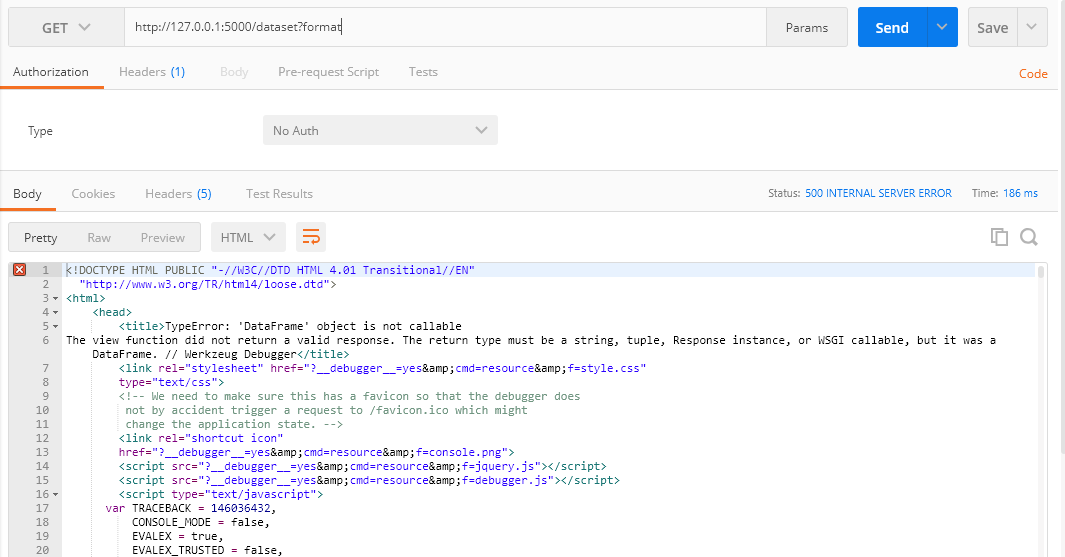
\includegraphics[width=0.85\textwidth]{figures/10/er1.PNG}}
	\caption{Error 1 untuk error 10 pada contoh kasus 3}
	\label{fig:er1}
\end{figure}

\item Maka tindakannya seperti berikut	:
\begin{itemize}
\item Perhatikan terlebih dahulu request yang diminta
\item Request yang diminta yaitu format
\item Silahkan diperiksa kembali apakah pada codingan API nya terdapat request global untuk parameter Format
\item Ada, namun harus disertai dengan parameter yang lain
\item Seperti ini : ?format=json
\item Ketika requestnya seperti itu, maka hasilnya akan muncul
\item Silahkan jalankan kembali requestnya
\item Maka hasilnya akan nampak seperti pada gambar \ref{fig:hu2}.
\begin{figure}[!htbp]
	\centerline{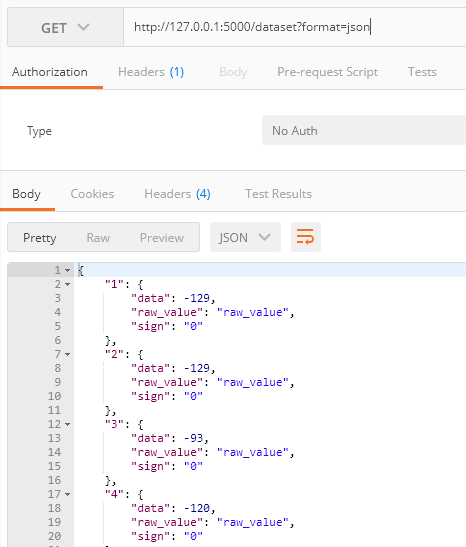
\includegraphics[width=0.85\textwidth]{figures/10/hu2.PNG}}
	\caption{Hasil pengujian 2 untuk error 10 pada contoh kasus 3}
	\label{fig:hu2}
\end{figure}
\end{itemize}
\end{enumerate}

\subsection{Error 3}
\begin{enumerate}
\item Silahkan jalankan kembali CMD anda
\item Kemudian masuk ke Directory tempat anda menyimpan file main.py
\item Kemudian masukkan perintah berikut : Env/scripts/activate
\item Maksud dari Code tersebut ialah untuk mengaktifkan scriptnya python3
\item Maka hasilnya akan nampak seperti pada gambar \ref{fig:am4}.
\begin{figure}[!htbp]
	\centerline{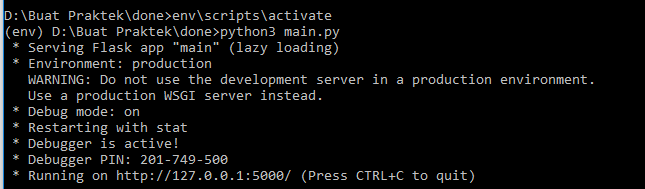
\includegraphics[width=0.85\textwidth]{figures/10/am4.PNG}}
	\caption{Aktivasi main.py 4 pada contoh kasus 3}
	\label{fig:am4}
\end{figure}

\item Apabila hasilnya seperti gambar diatas maka filenya telah berjalan dengan baik
\item Bisa dilihat, untuk URL APInya sudah muncul jadi silahkan copy dan buktikan menggunakan POSTMAN atau browser biasa.
\item Hasilnya seperti berikut, apabila dieksekusi sesuai endpoint.
 \item Misalnya endpoint : dataset/<id> seperti pada gambar \ref{fig:hu11}.
\begin{figure}[!htbp]
	\centerline{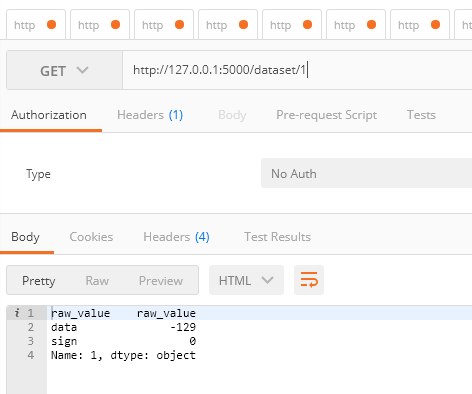
\includegraphics[width=0.85\textwidth]{figures/10/hu11.PNG}}
	\caption{Hasil pengujian 1 untuk error 11 pada contoh kasus 3}
	\label{fig:hu11}
\end{figure}

\item Kemudian apabila muncul ERROR seperti pada gambar \ref{fig:err11}.
\begin{figure}[!htbp]
	\centerline{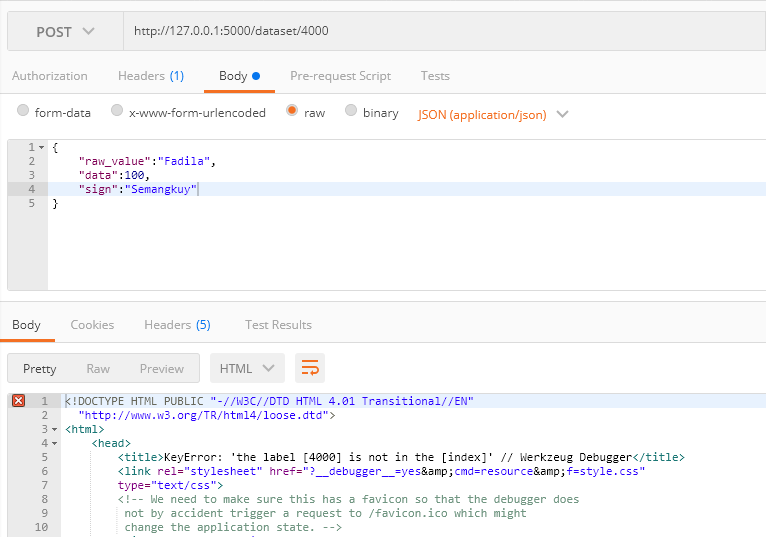
\includegraphics[width=0.85\textwidth]{figures/10/err11.PNG}}
	\caption{Error 1 untuk error 11 pada contoh kasus 3}
	\label{fig:err11}
\end{figure}

\item Maka tindakannya seperti berikut :
\begin{itemize}
\item Perhatikan terlebih dahulu request yang diminta
\item Request yang diminta yaitu id 4000
\item Silahkan diperiksa kembali apakah pada filenya ada id 4000 yang bisa diubah
\item Tidak ada, maka dari itu silahkan coba  diganti dengan id yang terdapat dala file tersebut
\item Seperti ini : dataset/2000
\item Ketika requestnya seperti itu maka hasilnya akan muncul
\item Silahkan jalankan kembali requestnya
\item Maka hasilnya akan nampak seperti pada gambar \ref{fig:hu21}.
\begin{figure}[!htbp]
	\centerline{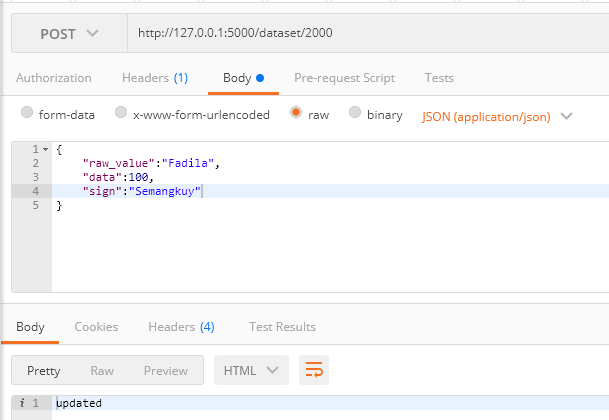
\includegraphics[width=0.85\textwidth]{figures/10/hu21.PNG}}
	\caption{Hasil pengujian 2 untuk error 11 pada contoh kasus 3}
	\label{fig:hu21}
\end{figure}
\end{itemize}

\item Maka id yang ke POST atau Update yaitu id 2000 dengan isi yang dapat diliat seperti pada gambar diatas.
\end{enumerate}